%:LLPStartPreview
%:VimtexCompile(SS)

%{{{ Formatierung

\documentclass[a4paper,12pt]{article}

\usepackage{physics_notetaking}

%%% dark red
%\definecolor{bg}{RGB}{60,47,47}
%\definecolor{fg}{RGB}{255,244,230}
%%% space grey
%\definecolor{bg}{RGB}{46,52,64}
%\definecolor{fg}{RGB}{216,222,233}
%%% purple
%\definecolor{bg}{RGB}{69,0,128}
%\definecolor{fg}{RGB}{237,237,222}
%\pagecolor{bg}
%\color{fg}

\newcommand{\td}{\,\text{d}}
\newcommand{\RN}[1]{\uppercase\expandafter{\romannumeral#1}}
\newcommand{\zz}{\mathrm{Z\kern-.3em\raise-0.5ex\hbox{Z} }}

\newcommand\inlineeqno{\stepcounter{equation}\ {(\theequation)}}
\newcommand\inlineeqnoa{(\theequation.\text{a})}
\newcommand\inlineeqnob{(\theequation.\text{b})}
\newcommand\inlineeqnoc{(\theequation.\text{c})}

\newcommand\inlineeqnowo{\stepcounter{equation}\ {(\theequation)}}
\newcommand\inlineeqnowoa{\theequation.\text{a}}
\newcommand\inlineeqnowob{\theequation.\text{b}}
\newcommand\inlineeqnowoc{\theequation.\text{c}}

\renewcommand{\refname}{Source}
\renewcommand{\sfdefault}{phv}
%\renewcommand*\contentsname{Contents}

\pagestyle{fancy}

\sloppy

\numberwithin{equation}{section}

%}}}

\begin{document}

%{{{ Titelseite

\title{physik311 $|$ Notizen}
\author{Jonas Wortmann}
\maketitle
\pagenumbering{gobble}

%}}}

\newpage

%{{{ Inhaltsverzeichnis

\fancyhead[L]{\thepage}
\fancyfoot[C]{}
\pagenumbering{arabic}

\tableofcontents

%}}}

\newpage

%{{{

\fancyhead[R]{\leftmark\\\rightmark}

\section{Einführung}
Licht ist eine elektromagnetische Welle. Die Wellenlänge ist im Bereich von $\SI{400}{nm}$ bis $\SI{800}{nm}$, das entspricht einer Frequenz von $\SI{750}{THz}$ bis $\SI{375}{THz}$. Ein Lichtpuls kann nie kürzer als ein Zyklus sein.

\subsection{Lichtquellen}
\begin{enumerate}[label=--]
        \item Lampe: Inkoherentes (\glqq ungeordnetes\grqq{}) Licht
        \item Laser: Koherentes (\glqq geordnetes\grqq{}, auch Wellen in \glqq gleichschritt\grqq{}) Licht
\end{enumerate}

\newpage
\section{Die elektromagnetische Theorie des Lichts}
Für diesen Fall betrachtet man nur die Lichtausbreitung in großer Entfernung von allen Quellen. Also ist $\rho =0$ und $\vv{j}=0$. Die \textsc{Maxwell}--Gleichungen sind dann
\begin{align}
        \,\text{div}\,\vv{D}&=0\\
        \,\text{div}\,\vv{B}&=0\\
        \,\text{rot}\,\vv{E}&=-\diffp[]{\vv{B}}{t}\\
        \,\text{rot}\,\vv{H}&=\diffp[]{\vv{D}}{t}
.\end{align}
In Materialien gilt dann
\begin{align} 
        \vv{D}&=\varepsilon \varepsilon _0\vv{E}\\
        \vv{B}&=\mu \mu _0\vv{H}
.\end{align} 
Hier ist $\varepsilon $ die Dielektrizitätskonstante und $\mu $ die relative Permeabilität (in der Optik ist sie üblicherweise 1). \\\indent
\begin{align} 
        \,\text{rot}\,\left(\,\text{rot}\,\vv{E}\right)&=\underbrace{\,\text{div}\,\left(\,\text{div}\,\vv{E}\right)}_{=0}-\left(\vv{\nabla }\cdot \vv{\nabla }\right)\vv{E}&&|\left(\vv{\nabla }\cdot \vv{\nabla }\right)=\,\text{div}\,\,\text{grad}\,=\triangle\\
                                                       &=\,\text{rot}\,\left(-\diffp[]{\vv{B}}{t}\right)
.\end{align} 
Mit $\,\text{rot}\,\vv{B}=\varepsilon\mu \varepsilon _0 \mu _0\diffp[]{\vv{E}}{t}$ folgt
\begin{align} 
        \triangle \vv{E}&=\varepsilon \mu \varepsilon _0\mu _0\diffp[2]{\vv{E}}{t}
.\end{align} 
Dies ist die \textbf{Wellengleichung} für das elektrische Feld. Man erwartet eine Ausbreitungsgeschwindigkeit mit
\begin{align} 
        v_{\,\text{ph}\,}&=\dfrac{1}{\,\sqrt[]{\varepsilon \mu \varepsilon _0\mu _0}}\equiv \dfrac{c}{n}
,\end{align} 
wobei $c=\,\sqrt[]{\varepsilon _0\mu _0}^{-1}$ die Vakuumslichtgeschwindigkeit und $n=\,\sqrt[]{\varepsilon \mu }$ der Brechungsindex ist. Dann lässt sich die Wellengleichung wie folgt schreiben
\begin{align} 
        \triangle \vv{E}&=\dfrac{1}{v_{\,\text{ph}\,}^2}\diffp[2]{\vv{E}}{t}\stackrel{\,\text{Vakuum}\,}{=}\dfrac{1}{c^2}\diffp[2]{\vv{E}}{t}
.\end{align} 
Eine analoge Rechnung kann auch für das $\vv{B}$--Feld verwendet werden.\\\indent

\subsection{Einfachste Lösung der Wellengleichung: Ebene elektromag.\ Welle}
Hier wird die Lichtausbreitung nur entlang einer Koordinate (z.B.\ $z$) betrachtet. Also ist $\vv{E}\left(\vv{r},t\right)=\vv{E}\left(z,t\right)$, bzw.\ $\diffp[]{\vv{E}}{x}=\diffp[]{\vv{E}}{y}=0$. Die Wellengleichung vereinfacht sich dann zu
\begin{align} 
        \diffp[2]{\vv{E}}{z}=\dfrac{1}{c^2}\diffp[2]{\vv{E}}{t}
.\end{align} 
Mit $\,\text{div}\,\vv{E}=0$ folgt für ebene Wellen $\diffp[]{E}{z}=0$, also ist $E_z=\,\text{const.}\,$.\\\indent
Jetzt wählt man die Randbedingungen, dass $E_z=0$. Also ist $\vv{E}=\begin{pmatrix}
        E_x\left(z\right)\\E_y\left(z\right)\\0
\end{pmatrix}$. Die Lösung der Wellengleichung ist dann
\begin{align} 
        \vv{E}\left(z,t\right)&=\vv{E}_0\cos \left(kz-\omega t\right)\\
                              &=\vv{E}_0\cos \left(k\left(z-ct\right)\right)
,\end{align} 
wobei $\tfrac{\omega }{k}=c$, mit $k=\tfrac{2\pi }{\lambda }$ der \textbf{Wellenzahl} ($\lambda $ der Wellenlänge) und $\vv{E}_0$ der Amplitude.\\\indent
Die Transversalität (also die Ausbreitung nach oben und unten, $\vv{E}\perp \vv{e}_z$, allg.\ $\vv{E}_z\perp \vv{k}$) folgt aus $\,\text{div}\,\vv{E}=0$ im ladungsfreien Raum. In Medien mit Raumladungen oder an Oberflächen ist auch eine longitudinale Polarisation möglich. Bisher gab es nur lineare Polarisationen; es ist aber auch eine Überlagerung von $E_x$ und $E_y$ möglich. Diese sind zirkulare und elliptische Polarisation.\\\indent
Die Allgemeine Wellengleichung ist
\begin{align} 
        \triangle \vv{E}=\left(\dfrac{n}{c}\right)^2\diffp[2]{\vv{E}}{t}
,\end{align} 
mit $v_{ph}=\tfrac{c}{n}$. Man erlaubt nun die Ausbreitung in eine beliebige Richtung sowie eine allgemeine Phase $\varphi $. Die Lösung ist dann
\begin{align} 
        \vv{E}\left(\vv{r},t\right)=\vv{E}_0\cos \left(\vv{k}\vv{r}-\omega t+\varphi \right)
.\end{align} 
Diese Gleichung erfüllt die Wellengleichung, wenn
\begin{align} 
        \vv{k}^2=\dfrac{n^2\omega ^2}{c^2}
.\end{align} 
Man bezeichnet sie auch als \textbf{Dispersionsrelation}.\\\indent
Aus den \textsc{Maxwell}--Gleichungen ist bekannt, dass
\begin{align} 
        \vv{B}=\dfrac{1}{\omega }\left(\vv{k}\times \vv{E}\right)
.\end{align} 
Das zeigt, dass $\vv{B}\perp \vv{E}\land \vv{k}$ und $|\vv{B}|=\tfrac{n}{c}|\vv{E}|$.\\\indent
Die Ursache der Wechselwirkung zwischen Licht und Materie ist überwiegend der elektrische Anteil der Welle (im sichtbaren Bereich).\\\indent
$\vv{E}$ und $\vv{B}$ sind nur im Fernfeld in Phase.

\subsection{Energie und Impuls von Licht}
Zuerst wird die Energiedichte des elektromagnetischen Feldes im Vakuum eingeführt
\begin{align} 
        W_{\,\text{el}\,}&=\dfrac{1}{2}\varepsilon _0E^2+\dfrac{1}{2}\dfrac{1}{\mu _0}B^2\qquad |\vv{B}|=\dfrac{1}{c}|\vv{E}|\qquad c=\dfrac{1}{\,\sqrt[]{\varepsilon _0\mu _0}}
.\end{align} 
Diese Gleichung wird zeitlich gemittelt, mit $E\left(t\right)=E_0\cos \left(\vv{k}\vv{r}-\omega t\right)$ und $\left\langle \cos ^2\right\rangle =\tfrac{1}{2}$
\begin{align} 
        \left\langle W_{\,\text{el}\,}\right\rangle =\dfrac{1}{2}\varepsilon _0E_0^2
.\end{align} 
Die mittlere Energiedichte, die pro Zeit durch ein Flächenelement transportiert wird ist
\begin{align} 
        I=c \left\langle W_{\,\text{el}\,}\right\rangle \qquad \left[I\right]=\dfrac{\SI{}{W}}{\SI{}{m^2}}
.\end{align} 
Die Richtung des Energietransports wird durch den \textsc{Poynting}--Vektor angegeben
\begin{align} 
        \vv{S}=\dfrac{1}{\mu _0}\vv{E}\times \vv{B}\qquad |\vv{S}|=\dfrac{1}{\mu _0}|\vv{E}||\vv{B}|=\varepsilon _0cE_0^2
.\end{align} 
Man erkennt, dass
\begin{align} 
        \left\langle |\vv{S}|\right\rangle =I
\end{align} 

\subsubsection{Strahlungsdruck}
Strahlungsdruck ist der Druck, der durch emittierte, absorbierte und reflektierte elektromagnetische Strahlung auf eine Fläche ausgeübt wird. Der Impuls von Teilchen mit der Geschwindigkeit $c$ ist
\begin{align} 
        p=\dfrac{E}{c}=\dfrac{A\cdot t\cdot c\cdot  \left\langle W_{\,\text{el}\,}\right\rangle }{c}
.\end{align} 
Der Druck ist $\rho =\tfrac{|\vv{F}|}{A}$ mit $|\vv{F}|=\diff[]{p}{t}$,
\begin{align} 
        \rho =\dfrac{I}{c}
.\end{align} 

%\newpage
\subsection{Elektromagnetische Wellen an Grenzflächen}
%\begin{wrapfigure}{L}{0.25\textwidth}
%        \centering
%        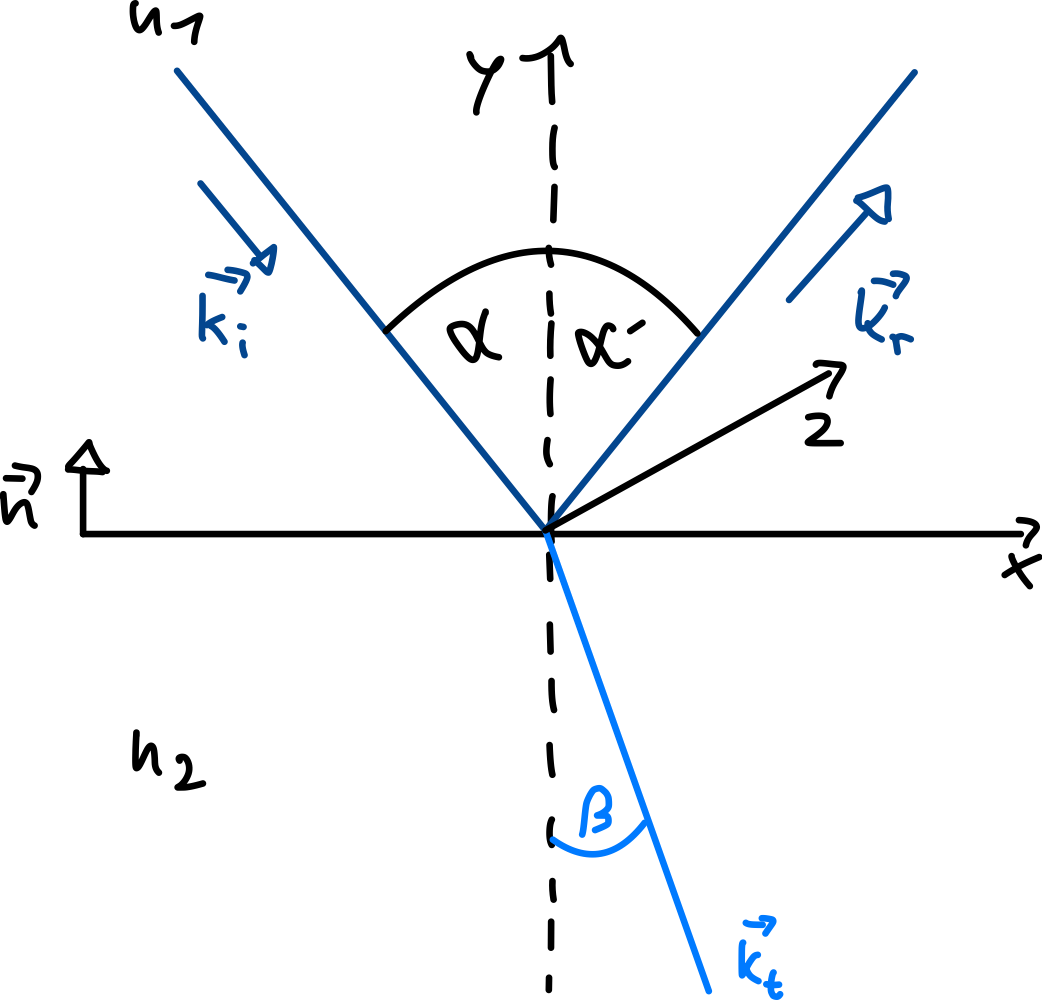
\includegraphics[width=0.25\textwidth]{Brechung.png}
%        \caption{asdf}
%\end{wrapfigure}
Lichtstrahl $\vv{k}_i$ trifft aus einem Medium $n_1$ in ein Medium $n_2>n_1$ und wird mit $\alpha $ zu $\vv{k}_r$ reflektiert. Das Licht wird auch um den Winkel $\beta $ gebrochen und verläuft mit $\vv{k}_t$ durch das Medium. Die $\vv{E}$--Felder sind dann
\begin{align} 
        \vv{E}_i&=\vv{E}_{0i}e^{\text{i}\left(\omega _it-\vv{k}_i\vv{r}\right)}\\
        \vv{E}_r&=\vv{E}_{0r}e^{\text{i}\left(\omega _rt-\vv{k}_r\vv{r}\right)}\\
        \vv{E}_t&=\vv{E}_{0r}e^{\text{i}\left(\omega _tt-\vv{k}_t\vv{r}\right)}
.\end{align} 
Das \textsc{Fermat}'sche Prinizp besagt, dass eine Welle immer den Weg der minimalsten optische Laufzeit wählt. Es ist also möglich, dass sie in einem Medium mehr Zeit verbringt, bevor sie in das andere Medium wechselt.

\subsubsection{Stetigkeit}
Die Tangentialkomponente von $\vv{E}$ und $\vv{H}=\tfrac{1}{\mu \mu _0}\vv{B}$ sind an Grenzflächen stetig. Die Normalkomponente von $\vv{D}=\varepsilon \varepsilon _0\vv{E}$ und $\vv{B}$ sind an Grenzflächen stetig.\\\indent
Zunächst werden die $\vv{E}$--Felder betrachtet, wenn $\vv{r}=0$ ist.
\begin{align} 
        \vv{n}\times \left(\vv{E}_{0i}e^{\text{i}\omega _it}+\vv{E}_{0r}e^{\text{i}\omega _rt}\right)\stackrel{!}{=}\vv{n}\times \vv{E}_{0t}e^{\text{i}\omega _tt}
.\end{align} 
Diese Gleichung muss für beliebige Zeiten $t$ gelten. Es existiert nur eine nichttriviale Lösung wenn $\omega _r=\omega _i=\omega _t\equiv \omega $.
\\\hfill\\\textbf{Einschub}\\ 
An allgemeinen Grenzflächen bleibt die Frequenz gleich, also $\omega _{\,\text{vac}\,}=\omega _{\,\text{medium}\,}$,
\begin{align} 
        E=E_0\cos \left(kz-\omega t\right)=E_0\cos \left[k\left(z-\dfrac{\omega }{k}t\right)\right]
,\end{align} 
mit $\tfrac{\omega }{k}=\tfrac{c}{n}=v_{\,\text{ph}\,}$, also 
\begin{align} 
k_{\,\text{vac}\,}=\tfrac{k_{\,\text{medium}\,}}{n}\Leftrightarrow \dfrac{2\pi }{\lambda _{\,\text{vac}\,}}=\dfrac{2\pi }{\lambda _{\,\text{medium}\,}}\dfrac{1}{n}\Leftrightarrow \lambda _{\,\text{Medium}\,}=\dfrac{1}{n}\lambda _{\,\text{vac}\,}
.\end{align} 
Daraus folgt, dass $\omega =k\tfrac{c}{n}$.\\\indent
Jetzt ist $\vv{r}$ ein beliebiger Punkt auf der Grenzfläche, also
\begin{align} 
        \left.e^{\text{i}\omega t}\vv{n}\times \left(\vv{E}_{0,i}e^{-\text{i}\vv{k}_i\vv{r}}+\vv{E}_{r,0}e^{-\text{i}\vv{k}_r\vv{r}}-\vv{E}_{t,0}e^{-\text{i}\vv{k}_t\vv{r}}\right)\right|_{y=0}=0
.\end{align} 
Es muss für beliebiges $\vv{r}$ auf der Grenzfläche gelten
\begin{align} 
        \vv{kk´}_i\vv{r}=\vv{k}_r\vv{r}=\vv{k}_t\vv{r}\,\forall \vv{r}=\begin{pmatrix}
                x\\0\\z
        \end{pmatrix}
.\end{align} 
Für das einfallende Lichtfeld setzt man
\begin{align} 
        \vv{k}_i=\begin{pmatrix}
                k_{i,x}\\k_{i,r}\\0
        \end{pmatrix}
.\end{align} 
Daraus folgt
\begin{align} 
        \begin{pmatrix}
                k_{i,x}\\k_{i,r}\\0
        \end{pmatrix}\cdot \begin{pmatrix}
                x\\0\\z
        \end{pmatrix}=\begin{pmatrix}
                k_{r,x}\\k_{r,y}\\k_{r,z}
        \end{pmatrix}\begin{pmatrix}
                x\\0\\z
        \end{pmatrix}=\begin{pmatrix}
                k_{z,x}\\k_{t,y}\\k_{t,z}
        \end{pmatrix}\begin{pmatrix}
                x\\0\\z
        \end{pmatrix}
.\end{align} 
Das heißt, auch die reflektierten und transmutierten Strahlen bleiben in der Zeichenebene. Das gilt auch für
\begin{align} 
        k_{r,x}&=k_{i,x}&k_r\sin \alpha '&=k_i\sin \alpha \\
        k_{t,x}&=k_{i,x}&k_t\sin \beta &=k_i\sin \alpha 
.\end{align} 
Da $\omega $ immer gleich ist, ist $\tfrac{k}{n}$ konstant. Mit $k_i=k_r$ folgt $\alpha '=\alpha $. Aus den Gleichungen folgt auch, dass 
\begin{align} 
        k_t&=\dfrac{n_2}{n_1}k_i&n_1\sin \alpha &=n_2\sin \beta 
.\end{align} 
Diese Gleichung ist das \textsc{Snellius}'sche Brechungsgesetz. Für $n_2>n_1$ wird der Strahl zum Lot hin gebrochen.

\subsubsection{Die Amplitude von reflektiertem und gebrochenen Strahl}
Hier wird nur der Spezialfall des senkrecht Einfallenden Strahls betrachtet. Es gilt
\begin{align} 
        \vv{E}_{0,i}+\vv{E}_{0,r}&=\vv{E}_{0,t}\\
        n_1\left(\vv{E}_{0,i}-\vv{E}_{0,r}\right)&=n_1\vv{E}_{0,t}\\
        \vv{B}_{0,i}+\vv{B}_{0,r}&=\vv{B}_{0,t}
.\end{align} 
Der Zusammenhang zwischen den Feldern ist
\begin{align} 
        \vv{B}&=\dfrac{1}{\omega }\left(\vv{k}\times \vv{E}\right)&\vv{k}_r&=-\vv{k}_i
.\end{align} 
Aus diesen Gleichungen folgt
\begin{align} 
        E_{0,r}&=\dfrac{n_1-n_2}{n_1+n_2}\vv{E}_{0,i}&r&=\dfrac{n_1-n_2}{n_1+n_2}
,\end{align} 
mit $r$ dem Reflexionskoeffizienten. Für $n_2>n_1$, id est eine Relexion am optisch dichteren Medium, ist $r<0$, daraus folgt ein Phasensprung von $\pi $. Das $\vv{E}$--Feld dreht sich also um. Die reflektierte Intensität ist
\begin{align} 
        R&=\dfrac{I_r}{I_i}=|r|^2=\left(\dfrac{n_1-n_2}{n_1+n_2}\right)^2
.\end{align} 
All das was nicht reflektiert, wird transmutiert
\begin{align} 
        |r|^2+|t|^2&=R+T=1&t&=\dfrac{E_{0,t}}{E_{0,r}}
.\end{align} 


%}}}

\end{document}
